\section{Dokumentation \& Doxygen}
\subsection{Dokumenation}
\subsubsection{Zweck der Dokumentation}
\begin{itemize}
	\item Wissenssicherung / Wissenstransfer
	\item Kommunikation
	\item Sichtbarkeit des Projektfortschritts
\end{itemize}
\subsubsection{Dokumenation von Software}
\begin{itemize}
	\item Schnittstellenbeschreibung (API)
	\item Zielgruppe ist Programmierer
	\item Dokumente werden oftmals nicht nachgeführt, wenn Änderungen am Sourcecode gemacht werden $\rightarrow$ Inkonsistenz
	\item Im Sourcecode wird mittels speziellem gekennzeichnetm Kommentar Beschreibung erstellt
	\item Mittels Dokumentationswerkzeugen kann Kommentar Source-Code extrahiert werden und daraus wird eine Beschreibung erstellt.  
\end{itemize}
\subsection{Doxygen}
Doxygen ist ein solches Dokumenationswerkzeugen wie oben erwähnt.\\
Es ist weit verbreitet und ist Open-Source. (Beispiel im Anhang)
\begin{itemize}
	\item unterstütze Sprachen: C,C++,Java, C\#,...
	\item Ausgabeformate: HTML; LaTex, RTF, XML,...
	\item auch UML-Diagramme möglich
	\item Command Line Tool
	\item existiert aber auch ein GUI und ein Eclipse-Plugin (Eclox, in Eclipse das Symbol @)
	\item benötigt Konfigurationsdatei Doxyfile 
	\item im File Doxyfile sind alle Einstellungen gespeicher was alles in die Dokumentation muss
\end{itemize}
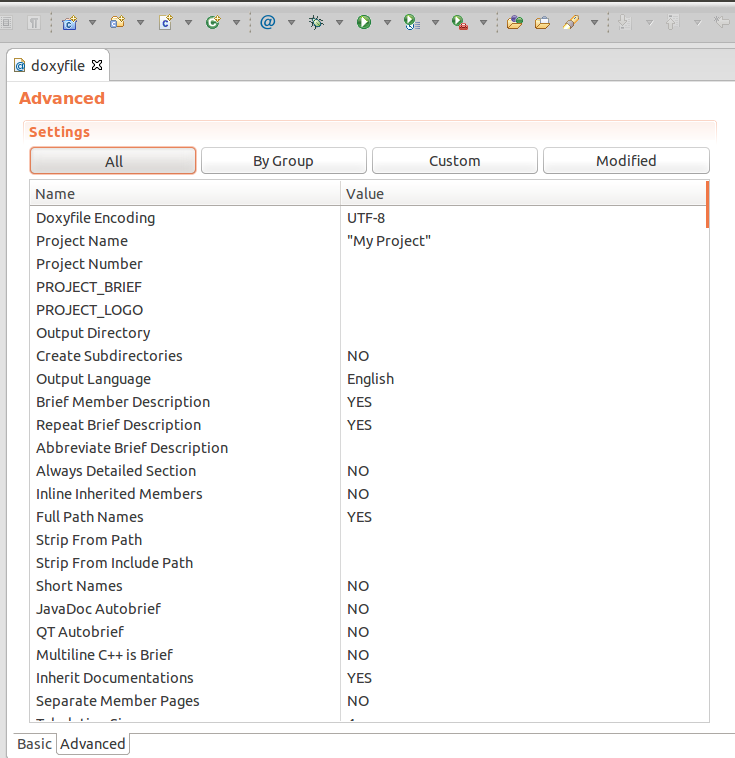
\includegraphics[width=9cm]{images/doxygen_advanced.png}
